\documentclass{article}

\def\subj {MATH}
\def\npart {304}
\def\nterm {Fall}
\def\nyear {2018}
\def\ncourse {Linear Algebra}


\input{header}



\setlength\parindent{0pt}

\begin{document}
\maketitle
{\small
  \noindent\textbf{Vectors and Matrices}\\
  Parameterised curves and arc length, tangents and normals to curves in $\R^3$, the radius of curvature.\hspace*{\fill} [1]

  \vspace{10pt}
  \noindent\textbf{Integration in $\R^2$ and $\R^3$}\\
  Line integrals. Surface and volume integrals: definitions, examples using Cartesian, cylindrical and spherical coordinates; change of variables.\hspace*{\fill} [4]

  \vspace{10pt}
  \noindent\textbf{Vector operators}\\
  Directional derivatives. The gradient of a real-valued function: definition; interpretation as normal to level surfaces; examples including the use of cylindrical, spherical *and general orthogonal curvilinear* coordinates.

  \vspace{5pt}
  \noindent Divergence, curl and $\nabla^2$ in Cartesian coordinates, examples; formulae for these operators (statement only) in cylindrical, spherical *and general orthogonal curvilinear* coordinates. Solenoidal fields, irrotational fields and conservative fields; scalar potentials. Vector derivative identities.\hspace*{\fill} [5]

  \vspace{10pt}
  \noindent\textbf{Integration theorems}\\
  Divergence theorem, Green's theorem, Stokes's theorem, Green's second theorem: statements; informal proofs; examples; application to fluid dynamics, and to electromagnetism including statement of Maxwell's equations.\hspace*{\fill} [5]

  \vspace{10pt}
  \noindent\textbf{Laplace's equation}\\
  Laplace's equation in $\R^2$ and $\R^3$: uniqueness theorem and maximum principle. Solution of Poisson's equation by Gauss's method (for spherical and cylindrical symmetry) and as an integral.\hspace*{\fill} [4]

  \vspace{10pt}
  \noindent\textbf{Cartesian tensors in $\R^3$}\\
  Tensor transformation laws, addition, multiplication, contraction, with emphasis on tensors of second rank. Isotropic second and third rank tensors. Symmetric and antisymmetric tensors. Revision of principal axes and diagonalization. Quotient theorem. Examples including inertia and conductivity.\hspace*{\fill} [5]}

\tableofcontents


\section{Vectors and Matrices}
\subsection{Fundamental Operations with Vectors}

	A vector $ \vec{v} \in \R^n $ is an ordered sequence of real numbers.
	\[
		\vec{v} = \begin{pmatrix} v_1 \\ v_2 \\ \vdots \\ v_n \end{pmatrix}
	\]
	
	The \textit{magnitude} (length) of a vector $ \vec{v} $ is $ ||\vec{v}|| = \sqrt{v_1^2 + v_2^2 + \dots + v_n^2} $. \\
	
	\textbf{Note}: If $ ||\vec{v}|| = 0 $, then $ \vec{v} = \vec{0} $.
	
	\subsubsection*{Scalar Multiplication}
	
	If $ c \in \R $ and $ \vec{v} = \begin{pmatrix} v_1 \\ v_2 \\ \vdots \\ v_n \end{pmatrix} \in \R^n $, then $ c\vec{v} = \begin{pmatrix} cv_1 \\ cv_2 \\ \vdots \\ cv_n \end{pmatrix} $. \\ \\
	
	\textbf{Note}: $ ||c\vec{v}|| = |c| \, ||\vec{v}|| $. \\
	
	Two non-zero vectors $ \vec{u}, \vec{v} $ are parallel if $ \vec{u} = c\vec{v} $ for some $ c \in \R $, $ c \neq 0 $. We can also infer that $ \vec{u} $ and $ \vec{v} $ have the same direction if $ c>0 $, and opposite direction if $ c<0 $.
	
	\subsubsection*{Vector Addition/Subtraction}
	
	If $ \vec{u} = \begin{pmatrix} u_1 \\ u_2 \\ \vdots \\ u_n \end{pmatrix}, \vec{v} = \begin{pmatrix} v_1 \\ v_2 \\ \vdots \\ v_n \end{pmatrix} $, then $ \vec{u} \pm \vec{v} = \begin{pmatrix} u_1 \pm v_1 \\ u_2 \pm v_2 \\ \vdots \\ u_n \pm v_n \end{pmatrix} $. \\ \\
	
	A vector $ \vec{v} \in \R^n $ is a linear combination of $ \vec{v}_1, \vec{v}_2, \dots, \vec{v}_k \in \R^n $ if
	\[
		\vec{v} = c_1 \vec{v}_1 + c_2 \vec{v}_2 + \dots + c_n \vec{v}_k
	\]
	where $ c_1,c_2,\dots,c_n \in \R $.
	
\subsection{The Dot Product}

	If $ \vec{u} = \begin{pmatrix} u_1 \\ u_2 \\ \vdots \\ u_n \end{pmatrix}, \vec{v} = \begin{pmatrix} v_1 \\ v_2 \\ \vdots \\ v_n \end{pmatrix} $, then the dot product of the vectors $ \vec{u} $ and $ \vec{v} $ is
	\[
		\vec{u} \cdot \vec{v} = \sum\limits_{k=1}^{n} u_k v_k = u_1v_1 + u_2v_2 + \dots + u_nv_n
	\]
	\textbf{Note}: $ \vec{u} \cdot \vec{u} = ||\vec{u}||^2 \geq 0 $.
	
	\subsubsection*{Cauchy-Schwartz Inequality}
	
	If $ \vec{u}, \vec{v} \in \R^n $, then
	\[
		|| \vec{u} \cdot \vec{v} || \leq || \vec{u} || \, || \vec{v}||
	\]
	\underline{Consequences}
	\begin{enumerate}[label=\arabic*.)]
		\item Triangle Inequality: If $ \vec{u},\vec{v} \in \R^n $, then $ || \vec{u} + \vec{v} || \leq ||\vec{u}|| + ||\vec{v}|| $.
		\begin{center}
			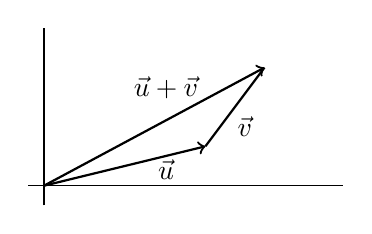
\begin{tikzpicture}
				\draw (0,0) -- (4,0);
				\draw (0.2,-0.25) -- (0.2,2);
				
				\draw [thick,->] (0.2,0) -- (3,1.5);
				\draw [thick,->] (0.2,0) -- (2.25,0.5);
				\draw [thick] (2.25,0.5) -- (3,1.5);
				
				\node at (1.75,1.25) {$\vec{u} + \vec{v}$};
				\node at (1.75,0.2) {$\vec{u}$};
				\node at (2.75, 0.75) {$\vec{v}$};
			\end{tikzpicture}
		\end{center}
		\begin{proof}
			\begin{align*}
				|| \vec{u} + \vec{v} ||^2 &= (\vec{u} + \vec{v}) \cdot (\vec{u} + \vec{v}) \\
				&= \vec{u} \cdot \vec{u} + \vec{u} \cdot \vec{v} + \vec{v} \cdot \vec{u} + \vec{v} \cdot \vec{v} \\
				&= || \vec{u} ||^2 + ||\vec{v}||^2 + 2(\vec{u} \cdot \vec{v}) \\
				&\geq ||\vec{u}||^2 + ||\vec{v}||^2 + 2||\vec{u}|| \, ||\vec{v}|| \\
				&= (||\vec{u}|| + ||\vec{v}||)^2
			\end{align*}
			Taking the square root we then obtain $ || \vec{u} + \vec{v} || \leq ||\vec{u}|| + ||\vec{v}|| $.
		\end{proof}
		\item Angle between $ \vec{u} $ and $ \vec{v} $: Defined as the number $ \theta \in [0,\pi] $ such that 
			\[
				\cos\theta = \frac{\vec{u} \cdot \vec{v}}{||\vec{u}|| \, ||\vec{v}||}
			\]
	\end{enumerate}

	\subsubsection*{Projection}
	
	The projection vector of $ \vec{b} $ onto $ \vec{a} $ is a vector $ \vec{p} $ parallel to $ \vec{a} $ such that $ \vec{b} - \vec{p} $ is orthogonal to $ \vec{a} $.
	
	\begin{center}
		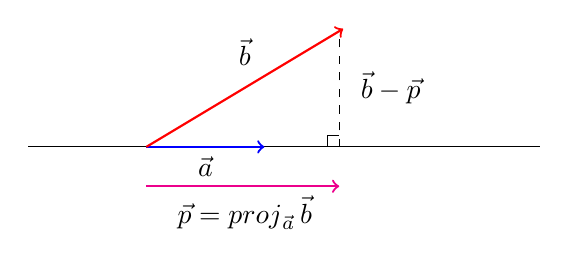
\begin{tikzpicture}
			\draw (0.5,0) -- (7,0);
			\draw[thick,->,blue] (2,0) -- (3.5,0);
			\draw[dashed] (4.45,0) -- (4.45,1.5);
			\draw (4.3,0) -- (4.3,0.15);
			\draw (4.3,0.15) -- (4.45,0.15);
			\draw[thick,->,red] (2,0) -- (4.5,1.5);
			\draw[thick,->,magenta] (2,-0.5) -- (4.45,-0.5);
			
			\node at (2.75,0) [below] {$\vec{a}$};
			\node at (3.25,-0.5) [below] {$\vec{p} = \text{proj}_{\vec{a}} \, \vec{b}$};
			\node at (3.25,1.2) {$\vec{b}$};
			\node at (4.6,0.75) [right] {$\vec{b} - \vec{p}$};
		\end{tikzpicture}
	\end{center}
	Thus the vector $ \vec{p} = c\vec{a} $ for some $ c > 0 \in \R $. Utilizing the geometry of the diagram, we can derive a formula for $ \text{proj}_{\vec{a}} \, \vec{b} $.
	\begin{align*}
		&(\vec{b} - \vec{p}) \cdot \vec{a} = 0 \\
		&\vec{b} \cdot \vec{a} = \vec{p} \cdot \vec{a} \\ 
		&\vec{b} \cdot \vec{a} = c \cdot \vec{a} \cdot \vec{a} \\ 
		&\vec{p} = \text{proj}_{\vec{a}} \, \vec{b} = \frac{\vec{a} \cdot \vec{b}}{|| \vec{a} ||^2} \vec{a}
	\end{align*}
	
	\textbf{Cauchy-Schwartz Inequality} \\
	
	If $ \vec{u}, \vec{v} \in \R^n $, then
	\[
		|| \vec{u} \cdot \vec{v} || \leq ||\vec{u}|| \, ||\vec{v}||
	\]
	\begin{proof}
		Consider the function $ f(t) = ||\vec{x} + t\vec{y}||^2 \leq 0 $. This is a quadratic polynomial in $ t $,
		\[
			||\vec{x} + t\vec{y}||^2 = ||\vec{y}||^2 t^2 + (2\vec{x} \cdot \vec{y}) t + ||\vec{x}||^2.
		\]
		Since this quadratic expression is always greater than or equal to 0, its discriminant must be less than or equal to 0, i.e,
		\begin{align*}
			&(2\vec{x} \cdot \vec{y} )^2 - 4(||\vec{y}||^2 \, ||\vec{x}||^2) \leq 0 \\
			&\Rightarrow 4(\vec{x} \cdot \vec{y})^2 \leq 4||\vec{y}||^2 \, ||\vec{x}||^2 \\
			&\Rightarrow \vec{x} \cdot \vec{y} \leq ||\vec{x}|| \, ||\vec{y}||
		\end{align*}
	\end{proof}

\subsection{Introduction to Proof Techniques}

	To prove the statement $ A \Rightarrow B $, we have the following proof techniques.

	\subsubsection*{Direct Proof}
	
	Logical step-by-step argument that starts from the given hypothesis and then concluding with the statement to be proved. 
	
	\begin{eg}
		Given $ \vec{x}, \vec{y} \in \R^n \, \backslash \{ \vec{0} \} $, prove that if $ \vec{x} \cdot \vec{y} \geq 0 $, then $ ||\vec{x} + \vec{y}|| \geq ||\vec{y}|| $.
		
		\begin{proof}
			Let us suppose that $ \vec{x} \cdot \vec{y} \geq 0 $. We first observe that $ ||\vec{x} + \vec{y}||^2 = ||\vec{x}||^2 + ||\vec{y}||^2 + 2(\vec{x} \cdot \vec{y}) $. Using our assumption, we get $ ||\vec{x} + \vec{y}||^2 \geq ||\vec{x}||^2 + ||\vec{y}||^2 $. Since $ \vec{x} \neq \vec{0} $, we get $ ||\vec{x} + \vec{y}||^2 > ||\vec{y}||^2 \Rightarrow ||\vec{x} + \vec{y}|| \geq ||\vec{y}|| $.
		\end{proof}
	\end{eg}

	\subsubsection*{Contrapositive Proof}
	
	To prove the statement $ A \Rightarrow B $, it is sufficient to prove that $ \neg B \Rightarrow \neg A $.
	
	\begin{eg}
		Prove $ \vec{x} \cdot \vec{y} \neq 0 \Rightarrow ||\vec{x} + \vec{y}||^2 \neq ||\vec{x}||^2 + ||\vec{y}||^2 $.
		
		\begin{proof}
			By contrapositive, it is sufficient to prove that $ ||\vec{x} + \vec{y}||^2 = ||\vec{x}||^2 + ||\vec{y}||^2 \Rightarrow \vec{x} \cdot \vec{y} = 0 $. Recall that $ ||\vec{x} + \vec{y}||^2 = ||\vec{x}||^2 + ||\vec{y}||^2 + 2(\vec{x} \cdot \vec{y}) $, from where we see that $ ||\vec{x} + \vec{y}||^2 = ||\vec{x}||^2 + ||\vec{y}||^2 $ implies that $ 2(\vec{x} \cdot \vec{y}) = 0 $, i.e, $ \vec{x} \cdot \vec{y} = 0 $.
		\end{proof}
	\end{eg}

	\subsubsection*{Proof by Contradiction}
	
	Assume $ A $, suppose $ B $ is false, then arrive at a contradiction, thus proving $ A \Rightarrow B $.
	
	\subsubsection*{If and Only If Proofs}
	
	This means that $ A \Rightarrow B $ \underline{and} $ B \Rightarrow A $ ($ A \Leftrightarrow B $). Also read that $ A $ is a necessary and sufficient condition for $ B $. To prove this, we need to prove each implication separately.
	
	\subsubsection*{Proof by Mathematical Induction}
	
	The objective is to prove that a statement $ P_n $ is true for the integer $ n \geq 0 $. \\
	
	\textbf{Strategy}
	\begin{itemize}
		\item  Verify the base case: $ P_0 $ is true.
		\item Prove the implication: $ P_n \Rightarrow P_{n+1} $.
		\item Conclude that $ P_n $ is true for all $ n \geq 0 $.
	\end{itemize}

	\begin{eg}
		Prove that 
		\[
			\sum\limits_{k=1}^{n} k^2 = \frac{n(n+1)(n+2)}{6} \quad n \in \Z^+
		\]
		for all $ n \geq 0 $.
		
		\begin{proof}
			By Mathematical induction on $ n \geq 1 $. \\
			
			Base case is true because
			\[
				\sum\limits_{k=1}^{1} 1^2 = 1 = \dfrac{1(1+1)(2(1)+1)}{6} .
			\]
			Let us now assume that the result holds up to $ n $ and let us prove that it holds for $ n+1 $.
			\begin{align*}
				\sum\limits_{k=1}^{n} k^2 &= \sum\limits_{k=1}^{n} k^2 + (n+1)^2 \\
				&= \frac{n(n+1)(n+2)}{6} + (n+1)^2 \\
				&= \frac{(n+1)(n(2n+1) + 6(n+1))}{6} \\
				&= \frac{(n+1)(2n^2 + 7n + 6)}{6} \\
				&= \frac{(n+1)(n+2)(2n+3)}{6} = \sum\limits_{k=1}^{n} (k+1)^2. 
			\end{align*}
			This shows that the result holds for $ n+1 $. We can conclude that $ P_n $ is true for all $ n \geq 1 $.
		\end{proof}
	\end{eg}
	
	\subsubsection*{Counterexamples}
	
	Used to disprove statements. \\
	
	We have seen that $ \vec{x} \cdot \vec{y} \geq 0 \Rightarrow ||\vec{x} + \vec{y}|| \geq ||\vec{y}|| $. What about the converse? Is it true that $ ||\vec{x} + \vec{y}|| > ||\vec{y}|| \Rightarrow \vec{x} \cdot \vec{y} \geq 0 $? \\
	
	No, a counterexample: $ \vec{x} = \begin{pmatrix} 5 \\0 \end{pmatrix}, \, \vec{y} = \begin{pmatrix} -1\\0 \end{pmatrix} $.
	
\subsection{Fundamental Operations with Matrices}

	\textbf{Matrix}: Rectangular array of real numbers arranged in $ m $ rows and $ n $ columns. Their size is denoted $ m \times n $. The set of all $ m \times n $ matrices is denoted by $ \R^{m \times n} $ or $ \mathcal{M}_{m \times n} $. \\
	
	To denote the entries of the matrix $ A \in \R^{m \times n} $ on the $ i^{th} $ row and $ j^{th} $ column, we write $ a_{ij} $.
	
	\subsubsection*{Diagonal Matrix}
	
	A matrix $ A $ is said to be diagonal if $ a_{ij} = 0 $ for any $ i \neq j $.
	\[
		\begin{pmatrix}
			a_{11} & 0      & \dots  & 0      \\
			0      & \ddots &        & \vdots \\
			\vdots &        & \ddots & 0      \\
			0      & \dots  & 0      & a_{ij}
		\end{pmatrix}
	\]
	
	\subsubsection*{Identity Matrix}
	
	Denoted by $ I_n $ where $ n $ is the number of columns.
	\[
		\begin{pmatrix}
			1      & 0      & \dots  & 0      \\
			0      & \ddots &        & \vdots \\
			\vdots &        & \ddots & 0      \\
			0      & \dots  & 0      & 1
		\end{pmatrix}
	\]
	
	\subsubsection*{Upper Triangular Matrix}
	
	A matrix $ A $ is said to be upper triangular if $ a_{ij} = 0 $ for any $ i>j $.
	\[
		\begin{pmatrix}
			a_{11} &        &        &        \\
			0      & \ddots &        &        \\
			\vdots &        & \ddots &        \\
			0      & \dots  & 0      & a_{ij}
		\end{pmatrix}
	\]
	
	\subsubsection*{Lower Triangular Matrix}
	
	A matrix $ A $ is said to be lower triangular if $ a_{ij} = 0 $ for any $ i<j $.
	\[
		\begin{pmatrix}
			a_{11} & 0      & \dots  & 0      \\
			       & \ddots &        & \vdots \\
			       &        & \ddots & 0      \\
			       &        &        & a_{ij}
		\end{pmatrix}
	\]
	
	\subsubsection*{Transpose}
	
	The transpose of a matrix $ A \in \R^{m \times n} $ is the matrix $ A^T \in \R^{n \times m} $ with entries
	\[
		(A^T)_{ij} = a_{ji}
	\]
	
	A square matrix $ A \in \R^{m \times n} $ is called
	\begin{itemize}
		\item \textit{Symmetric} if $ A^T = A $, i.e, $ a_{ji} = a_{ij} $.
		\item \textit{Skew-Symmetric} if $ A^T = -A $, i.e, $ a_{ji} = -a_{ij} $.
	\end{itemize}
	
	\begin{remark}
		The diagonal entries of a skew-symmetric matrix are equal to 0.
	\end{remark}

	\begin{thm}
		Every square matrix $ A \in \R^{n \times n} $ can be written in a unique way as the form of a symmetric matrix and a skew-symmetric matrix.
	\end{thm}

	\begin{proof} $ $ \vspace{2mm}\\
		\underline{Uniqueness}: Suppose that $ A = S+V $ where $ S $ is symmetric and $ V $ is skew-symmetric. We want to establish that $ S $ and $ V $ are uniquely determined.
		\begin{align*}
			A &= S+V \\
			A^T &= S^T + V^T \\
				&= S-V
		\end{align*}
		so $ A+A^T = 2S $ and $ A-A^T = 2V $, i.e, $ S = \frac{1}{2}(A+A^T) $, $ V = \frac{1}{2}(A-A^T) $. \\
		
		\underline{Existence}: For the fact that $ A $ can indeed be written as a sum of symmetric and skew-symmetric matrices, notice that
		\[
			A = \frac{A+A^T}{2} + \frac{A-A^T}{2}
		\]
		and that 
		\begin{align*}
			&\left( \frac{A + A^T}{2} \right)^T = \frac{A^T + (A^T)^T}{2} = \frac{A^T + A}{2} = \frac{A + A^T}{2}, \\
			&\left( \frac{A - A^T}{2} \right)^T = \frac{A^T - (A^T)^T}{2} = \frac{A^T - A}{2} = -\frac{A-A^T}{2}
		\end{align*}
	\end{proof}

	\subsection{Matrix Multiplication}
	
	The product of a matrix $ A \in \R^{m \times n} $ and $ B \in \R^{n \times p} $ is the matrix $ C = AB \in \R^{m \times p} $ with entries
	\[
		c_{ij} = \sum\limits_{k=1}^{n} a_{ik} b_{kj}
	\]
	
	\begin{remark} $  $ \vspace{1mm}
		\begin{itemize}
			\item This also defines a matrix-vector product since a vector is a matrix with 1 column.
			\item $ A\vec{x} = x_1 \col_1(A) + x_2 \col_2(A) + \dots + x_n \col_n(A) $
			\item $ A[\vec{b}_1 | \vec{b}_2 | \dots | \vec{b}_p] = [A\vec{b}_1 | A\vec{b}_2 | \dots | A\vec{b}_p] $
		\end{itemize}
	\end{remark}

	\begin{prop}
		If $ A \in \R^{m \times n}, B \in \R^{n \times p} $, then 
		\[
			(AB)^T = A^T B^T
		\]
	\end{prop}

	\begin{proof}
		\begin{align*}
			&((AB)^T)_{ij} = (AB)_{ji} = \sum\limits_{k=1}^{n} a_{jk} b_{ki} \\
			&(B^T A^T)_{ij} = \sum\limits_{k=1}^{n} (B^T)_{ik} (A^T)_{kj} = \sum\limits_{k=1}^{n} b_{ki} a_{jk}
		\end{align*}
	\end{proof}

	\section{Systems of Linear Equations}
	
	\subsection{Solving Linear Systems Using Gaussian Elimination}
	
	A linear systems of $ m $ equations and $ n $ unknowns is described as,
	\begin{alignat*}{2}
		&a_{1,1} x_1 + a_{1,2} x_2 + \dots + a_{1,n} x_n = &&b_1 \\
		&\vdots  &&\vdots \\
		&a_{m,1} x_1 + a_{m,2} x_2 + \dots + a_{m,n} x_n = \, &&b_m
	\end{alignat*}
	This is better represented in matrix form,
	\[
		\begin{bmatrix} a_{11} & a_{12} & \dots & a_{1n} \\ \vdots & \vdots & & \vdots \\ a_{m1} & a_{m2} & \dots & a_{mn} \end{bmatrix} \begin{bmatrix} x_1 \\ \vdots \\ x_n \end{bmatrix} = \begin{bmatrix} b_1 \\ \vdots \\ b_n \end{bmatrix}
	\]
	or just $ A\vec{x} = \vec{b} $. \\
	
	A linear system of the form $ A\vec{x} = \vec{b} $ with $ \vec{b} = \vec{0} $ is called a \textit{homogeneous} system. It will always have a solution $ \vec{x} = \vec{0} $, called the \textit{trivial solution}, but it may have other solutions called \textit{non-trivial}. \\
	
	In general, a linear system has either
	\begin{itemize}
		\item No solutions
		\item 1 unique solution
		\item Infinitely many solutions
	\end{itemize}

	Using only row operations, one can transform any linear system $ A\vec{x} = \vec{b} $, equivalently written in augmented form as $ [A | \vec{b}] $ into \textit{row-echelon form}, which can be solved using back substitution.
	
	\begin{eg}
		Find the cubic equation $ y = ax^3 + bx^2 + cx + d $ that goes through the points $ (1,2), (2,-12), (-2,56), (3,-54) $. \\
		
		We need to find $ a,b,c,d \in \R $ such that 
		\begin{align*}
			a + b + c + d &= 2 \\
			8a + 4b + 2c + d &= -12 \\
			-8a + 4b - 2c + d &= 56 \\
			27a + 9b + 3c + d &= -54
		\end{align*}
	Set the vector $ \begin{pmatrix} x_1 \\ x_2 \\ x_3 \\ x_4 \end{pmatrix} = \begin{pmatrix} d \\ c \\ b \\ a \end{pmatrix} $ and write the linear system in augmented form as
		\begin{align*}
			\begin{sysmatrix}{cccc|c}
				1 &  1 & 1 & 1 & 2 \\
				1 &  2 & 4 & 8 & -12 \\
				1 & -2 & 4 & -8 & 56 \\
				1 & 3 & 9 & 27 & 54
			\end{sysmatrix}
				&\!\begin{aligned}
				&\ro{r_2 \leftarrow r_2-r_1}\\
				&\ro{r_3 \leftarrow r_3 - r_1} \\
				&\ro{r_4 \leftarrow r_4 - r_1}
			\end{aligned}
			\begin{sysmatrix}{cccc|c}
				1 & 1 & 1 & 1 & 2 \\
				0 & 1 & 3 & 7 & -14 \\
				0 & -3 & -3 & -9 & 54 \\
				0 & 2 & 8 & 26 & -56
			\end{sysmatrix}
			\\
				&\!\begin{aligned}
				&\ro{r_3 \leftarrow (1/3)r_3}\\
				&\ro{r_4 \leftarrow (1/2)r_4}
				\end{aligned}
			\begin{sysmatrix}{cccc|c}
				1 & 1 & 1 & 1 & 2 \\
				0 & 1 & 3 & 7 & -14 \\
				0 & -1 & 1 & -3 & 18 \\
				0 & 1 & 4 & 13 & -28
			\end{sysmatrix}
			\\
			&\!\begin{aligned}
				&\ro{r_3 \leftarrow r_3 + r_2}\\
				&\ro{r_4 \leftarrow r_4 - r_2}
			\end{aligned}
			\begin{sysmatrix}{cccc|c}
				1 & 1 & 1 & 1 & 2 \\
				0 & 1 & 3 & 7 & -14 \\
				0 & 0 & 4 & 4 & 4 \\
				0 & 0 & 1 & 6 & -14
			\end{sysmatrix}
			\\
			&\ro{r_3 \leftarrow (1/4)r_3}
			\begin{sysmatrix}{cccc|c}
				1 & 1 & 1 & 1 & 2 \\
				0 & 1 & 3 & 7 & -14 \\
				0 & 0 & 1 & 1 & 1 \\
				0 & 0 & 0 & 1 & -14
			\end{sysmatrix}
			\\
			&\ro{r_4 \leftarrow r_4-r_3}
			\begin{sysmatrix}{cccc|c}
				1 & 1 & 1 & 1 & 2 \\
				0 & 1 & 3 & 7 & -14 \\
				0 & 0 & 1 & 1 & 1 \\
				0 & 0 & 0 & 5 & -15
			\end{sysmatrix}
			\\
			&\ro{r_4 \leftarrow (1/5)r_4}
			\begin{sysmatrix}{cccc|c}
				1 & 1 & 1 & 1 & 2 \\
				0 & 1 & 3 & 7 & -14 \\
				0 & 0 & 1 & 1 & 1 \\
				0 & 0 & 0 & 1 & -3
			\end{sysmatrix}
		\end{align*}
		Now that we have our matrix in row-echelon form, we can perform back substitution to find $ a,b,c,d $.
		\begin{align*}
			&x_4 = -3 \\
			&x_3 + x_4 = 1 \Rightarrow x_3 = 4 \\
			&x_2 + 3x_3 + 7x_4 = -14 \Rightarrow x_2 = -5 \\
			&x_1 + x_2 + x_3 + x_4 = 2 \Rightarrow\ x_1 = 6
		\end{align*}
		So $ a=-3, b=4, c=-5, d=6 $. Thus the equation of our cubic is
		\[
			y = -3x^3 + 4x^2 - 5x + 6
		\]
		If we apply further row operations, we can create zeros above the main diagonal, arriving at \textit{reduced row-echelon form}, which simplifies the back substitution.
		\begin{align*}
			\begin{sysmatrix}{cccc|c}
				1 & 1 & 1 & 1 & 2 \\
				0 & 1 & 3 & 7 & -14 \\
				0 & 0 & 1 & 1 & 1 \\
				0 & 0 & 0 & 1 & -3
			\end{sysmatrix}
			&\!\begin{aligned}
				&\ro{r_1 \leftarrow r_1 - r_4}\\
				&\ro{r_2 \leftarrow r_2 - 7r_4}\\
				&\ro{r_3 \leftarrow r_3 - r_4}
			\end{aligned}
			\begin{sysmatrix}{cccc|c}
				1 & 1 & 1 & 0 & 5 \\
				0 & 1 & 3 & 0 & 7 \\
				0 & 0 & 1 & 0 & 4 \\
				0 & 0 & 0 & 1 & -3
			\end{sysmatrix}
			\\
			&\!\begin{aligned}
				&\ro{r_1 \leftarrow r_1 - 7r_3} \\
				&\ro{r_2 \leftarrow r_2 - 3r_3}
			\end{aligned}
			\begin{sysmatrix}{cccc|c}
				1 & 1 & 0 & 0 & 1 \\
				0 & 1 & 0 & 0 & -5 \\
				0 & 0 & 1 & 0 & 4 \\
				0 & 0 & 0 & 1 & -3
			\end{sysmatrix}
			\\
			&\ro{r_1 \leftarrow r_1 - r_2}
			\begin{sysmatrix}{cccc|c}
				1 & 0 & 0 & 0 & 6 \\
				0 & 1 & 0 & 0 & -5 \\
				0 & 0 & 1 & 0 & 4 \\
				0 & 0 & 0 & 1 & -3
			\end{sysmatrix}
		\end{align*}
		Thus $ a=-3,b=4,c=-5,d=6 $.
	\end{eg}

	\begin{remark}
		Number of solutions to a linear system $ A\vec{x} = \vec{b} $ with reduced row echelon form $ C $.
		\begin{enumerate}[label=\alph*.)]
			\item If $ C $ has a row $ [0 \dots 0 | c_1] $ with $ c \neq 0 $, then we have no solutions.
			\item If $ C $ has a non-pivot column, then we have infinitely many solutions.
			\item Otherwise, we have a unique solution.
		\end{enumerate}
	\end{remark}

	\begin{cor}
		In a homogeneous linear system with fewer equations than unknowns $ (m<n) $, there is always a ``step" of size $ \geq 2 $.
	\end{cor}








	


\end{document}